
%------------------------------------------------   
\section{Data Analysis}





%------------------------------------------------   
\subsection{Obtención de los productos químicos más frecuentes en los cosméticos}

La obtención de los productos químicos más frecuentes en los cosméticos se va a realizar realizando histogramas sobre el campo \code{CasId} del dataset. La Figura \ref{fig:histogram-casid-basic} muestra el histograma sobre todo el dataset, donde se puede observar que entre los valores 600 y 700 hay un gran volumen. \\

Concretamente, este volumen se encuentra entre los valores 656 and 658. La Figura \ref{fig:histogram-casid-656-658} muestra el histograma entre dichos valores, donde se puede observar que el volumen se encuentra en el producto químico con \code{CasId} 656, cuyo nombre es: 
\begin{itemize}
 \item \code{656 - Titanium dioxide}
\end{itemize}

y pertenece al Cluster 0. 

\newpage
\begin{figure}[!th]
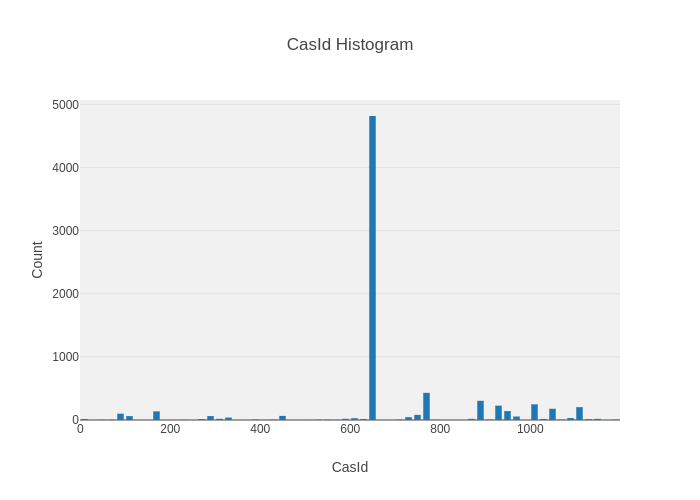
\includegraphics[scale=0.5]{figures/histogram-casid-basic}
\centering
\caption{Histograma sobre el campo \code{CasId}.}
\label{fig:histogram-casid-basic}
\end{figure}

\begin{figure}[!th]
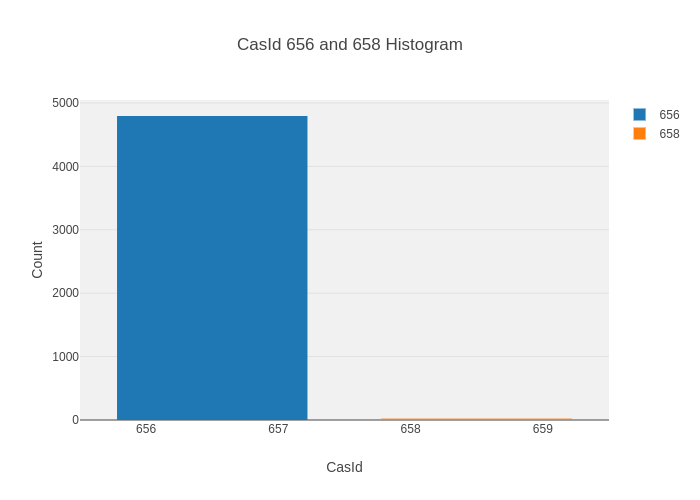
\includegraphics[scale=0.5]{figures/histogram-casid-656-658}
\centering
\caption{Histograma de los valores 656 y 658 del campo \code{CasId}.}
\label{fig:histogram-casid-656-658}
\end{figure}


Sin embargo, como podemos observar en la Figura \ref{fig:histogram-casid-basic}, la diferencia de volumen es muy grande entre el \code{CasId} 656 y el resto. Por lo que se va a realizar los mismos pasos anteriores, pero quitando el \code{CasId} 656 de los datos. \\

La Figura \ref{fig:histogram-casid-without656} muestra el histograma sobre el campo \code{CasId} del dataset sin el \code{CasId} 656 y, además, diferenciando por cluster, donde se puede observar que sigue habiendo un gran volumen entre los valores 700 y 800 y que pertenecen al Cluster 0.


\newpage
\begin{figure}[!th]
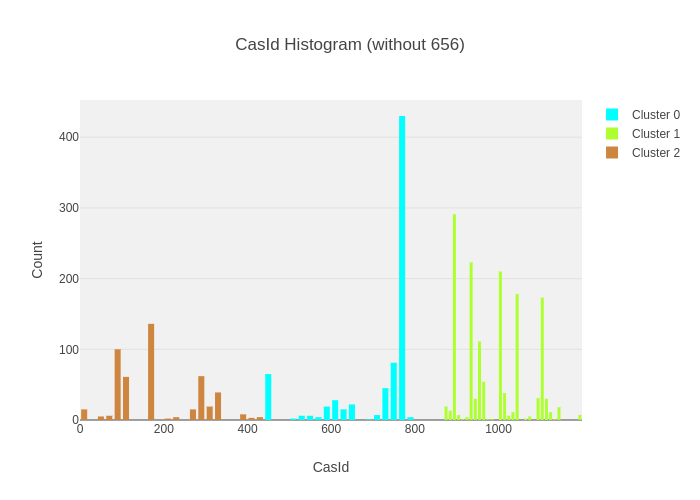
\includegraphics[scale=0.5]{figures/histogram-casid-without656}
\centering
\caption{Histograma sobre el campo \code{CasId} sin el \code{CasId} 656.}
\label{fig:histogram-casid-without656}
\end{figure}

Concretamente, este volumen se encuentra entre los valores 773 y 776. La Figura \ref{fig:histogram-casid-773-776} muestra el histograma entre dichos valores, donde se puede apreciar que el \code{CasId} 773 tiene mayor volumen. El nombre de cada uno de los productos químicos es:

\begin{itemize}
 \item \code{773 - Retinol/retinyl esters, when in daily dosages in excess of 10,000 IU, or 3,000 retinol equivalents}
 \item \code{776 - Silica, crystalline (airborne particles of respirable size)}
\end{itemize}

\begin{figure}[!th]
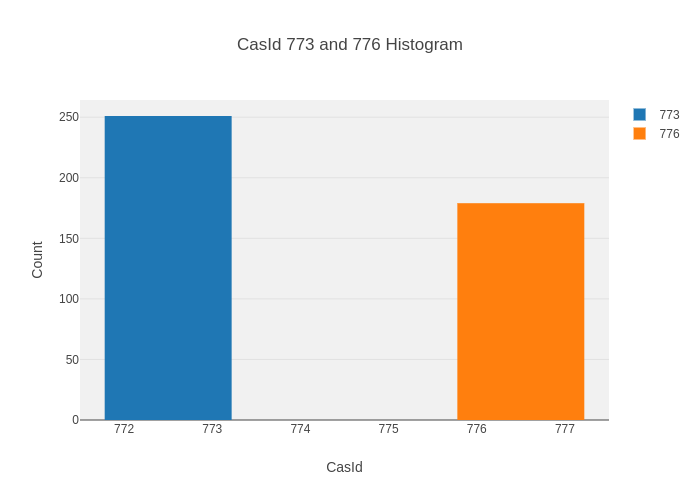
\includegraphics[scale=0.5]{figures/histogram-casid-773-776}
\centering
\caption{Histograma de los valores 773 y 776 del campo \code{CasId}.}
\label{fig:histogram-casid-773-776}
\end{figure}




\newpage

%------------------------------------------------   
\subsection{Obtención de los cosméticos con mayor número de productos químicos}



















\newpage
































